
\section{Rückblick}

\begin{frame}
  {Erinnerung an letzte Woche: segmentale Phonologie}
  \pause
  \begin{itemize}[<+->]
    \item Verteilungen: [\alert{z}oːlə] vs.\ [ʃmɪ\alert{s}]
    \item Neutralisierung:
      \begin{itemize}[<+->]
        \item  Weg [veː\rot{k}], Weges [veː\alert{g}əs]
        \item Bock [bɔ\rot{k}], Bockes [bɔ\alert{k}əs]
      \end{itemize}
    \item zugrundeliegende Formen und Strukturbedingungen (Beispiel)
      \begin{itemize}[<+->]
        \item /ăn/ $\Rightarrow$ [ʔan]
        \item /onə/ $\Rightarrow$ [ʔoːnə] 
      \end{itemize}
    \item Gespanntheit
      \begin{itemize}[<+->]
        \item \alert{gespannt = längbar} und \alert{ungespannt = nicht längbar}
        \item \alert{/ə/ unbetonbar und damit unlängabr}
        \item Kernwortschatz: entweder \alert{gespannt + betont + lang} [ʔoːfən]\\
          oder \alert{ungespannt + kurz} (und Betonung egal) [ʔɔfən]
        \item erweiterter Wortschatz: \alert{nur} \alert{gespannt + betont $\Rightarrow$ lang}: [ʔuʁaːn]
        \item ungespannte Vokale: \rot{immer} kurz: [fʏlt], *[fʏːlt]
      \end{itemize}
  \end{itemize}
\end{frame}



\section{Phonologie: Silben}

\begin{frame}
  {Übersicht}
  \pause
  \begin{itemize}[<+->]
    \item Silben als Organisationseinheiten für Segmente
    \item Silben als Mund-Öffnen-Schließen
    \item \alert{Sonorität} als die diesem entsprechende phonologische Größe
    \item Positionen in der Silbe und dort jeweils mögliche Segmente
    \item Einsilbler, Zweisilbler und das \alert{Silbengewicht}
    \item \alert{Silbengelenke}
      \Zeile
    \item Literatur: \rot{\citet{Eisenberg2013a}}, \citet{Maas2002}
  \end{itemize}
\end{frame}


\begin{frame}
  {Bezug der Silbenphonologie zum Lehrberuf}
  \pause
  \centering
  \LARGE
  \rot{Die Klatschmethode funktioniert nicht!}\\
  \pause
  \Zeile
  \rot{\ldots und die Hinhörschreibung auch nicht.}
\end{frame}


\begin{frame}
  {Was sind Silben?}
  \pause
  \begin{itemize}[<+->]
    \item genaue Definition schwierig
    \item "`rhythmische Einheiten"' (bzw.\ metrische Einheiten)
      \Zeile
    \item \alert{rein phonologische} Ebene \alert{zwischen Segment und Wort}
    \item eigene \alert{Regularitäten}: Abfolge der Segmente
      \Zeile
    \item \alert{nicht lexikalisch}: \textit{klüger} [klyː.g\rot{ɐ}], \textit{klügere} [klyː.g\rot{ə}.\rot{ʁ}ə]
  \end{itemize}
\end{frame}

\begin{frame}
  {Hinweis}
  \pause
  \Zeile\Zeile
  \centering
  \Large /ʁ/ und /l/ werden als \alert{Liquide} zusammengefasst.
\end{frame}


\begin{frame}[fragile]
  {Sonorität und Sonoritätshierarchie}
  \pause
  \begin{itemize}[<+->]
    \item \textit{Tag}, \textit{Mund}, \textit{Lob}, \textit{Knack}, \textit{grün}, \textit{Klang}, \dots
      \Zeile
    \item Prototypisch:
      \begin{itemize}[<+->]
        \item \alert{Sprechwerkzeuge öffnen und schließen}
        \item \alert{Stimmton geht an und aus.}
      \end{itemize}
      \Zeile
    \item unterschiedliche Öffnungsgrade bei Plosiven, Frikativen, Lateralen,\\
      Nasalen, Vokalen entsprechen ungefähr der \alert{Sonorität}
  \end{itemize}
  \pause
  \begin{center}
    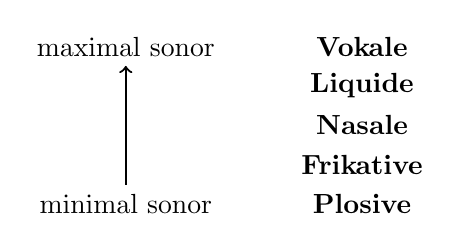
\begin{tikzpicture}
      \node (min)                             {minimal sonor};
      \node (plo) at ([shift={( 3,0)}]   min) {\textbf{Plosive}};
      \node (fri) at ([shift={( 0,0.5)}] plo) {\textbf{Frikative}};
      \node (nas) at ([shift={( 0,0.5)}] fri) {\textbf{Nasale}};
      \node (liq) at ([shift={( 0,0.5)}] nas) {\textbf{Liquide}};
      \node (vok) at ([shift={( 0,0.5)}] liq) {\textbf{Vokale}};
      \node (max) at ([shift={(-3,0)}]   vok) {maximal sonor};
      \draw [->, thick] (min) to (max);
    \end{tikzpicture}
  \end{center}
\end{frame}


\begin{frame}[fragile]
  {Sonoritätskonturen}
  \pause
  \begin{center}
      \SonDiag[2]{{k/\plo/0, u:/\vok/0}}
  \end{center}
\end{frame}

\begin{frame}[fragile]
  {Sonoritätskonturen}
  \begin{center}
      \SonDiag[2]{{n/\nas/0, i:/\vok/0}}
  \end{center}
\end{frame}

\begin{frame}[fragile]
  {Sonoritätskonturen}
  \begin{center}
      \SonDiag[3]{{k/\plo/0, n/\nas/0, i:/\vok/0}}
  \end{center}
\end{frame}

\begin{frame}[fragile]
  {Sonoritätskonturen}
  \begin{center}
      \SonDiag[3]{{d/\plo/0, ʁ/\liq/0, oː/\vok/0}}
  \end{center}
\end{frame}

\begin{frame}[fragile]
  {Sonoritätskonturen}
  \begin{center}
      \SonDiag[3]{{ʃ/\fri/2, t/\plo/0, e:/\vok/0}}
  \end{center}
\end{frame}

\begin{frame}[fragile]
  {Sonoritätskonturen}
  \begin{center}
      \SonDiag[4]{{ʃ/\fri/2, p/\plo/0, ʁ/\liq/0, y:/\vok/0}}
  \end{center}
\end{frame}

\begin{frame}[fragile]
  {Sonoritätskonturen}
  \begin{center}
      \SonDiag[3]{{ʔ/\plo/0, a/\vok/0, p/\plo/0}}
  \end{center}
\end{frame}

\begin{frame}[fragile]
  {Sonoritätskonturen}
  \begin{center}
      \SonDiag[3]{{ʔ/\plo/0, a/\vok/0, n/\nas/0}}
  \end{center}
\end{frame}

\begin{frame}[fragile]
  {Sonoritätskonturen}
  \begin{center}
      \SonDiag[4]{{ʔ/\plo/0, a/\vok/0, χ/\fri/0, t/\plo/0}}
  \end{center}
\end{frame}

\begin{frame}[fragile]
  {Sonoritätskonturen}
  \begin{center}
      \SonDiag[4]{{ʔ/\plo/0, a/\vok/0, l/\liq/0, m/\nas/0}}
  \end{center}
\end{frame}

\begin{frame}[fragile]
  {Sonoritätskonturen}
  \begin{center}
      \SonDiag[4]{{ʁ/\liq/0, a/\vok/0, p/\plo/0, s/\fri/2}}
  \end{center}
\end{frame}


\begin{frame}[fragile]
  {Silbenstruktur, konstruiert am Einsilbler}
  \pause
  Im Einsilbler:\\
  \begin{itemize}[<+->]
    \item \rot{immer ein Vokal}
    \item \alert{immer mindestens ein Konsonant davor (ggf.\ [ʔ])}
    \item möglicherweise Konsonanten danach\\
      (ohne: \alert{offene} Silbe, mit: \alert{geschlossene} Silbe)
    \item Diagramm der maximalen Silbenstruktur im Deutschen:
  \end{itemize}
  \pause
  \begin{center}
    \begin{forest}
      [Silbe, calign=last
        [Anfangsrand, sake, calign=first
          [C][C]
        ]
        [Reim, calign=first
          [Kern, sake, calign=first
            [V]
          ]
          [Endrand, sake, calign=last
            [C][C]
          ]
        ]
      ]
    \end{forest}
  \end{center}
\end{frame}


\begin{frame}[fragile]
  {Extrasilbisch I}
  \pause
  \begin{itemize}[<+->]
    \item eingekreist: \alert{Verletzungen der Sonoritätskontur}
    \item Lösung: nicht i.\,e.\,S.\ Bestandteile der Silben
    \item \rot{extrasilbische} Konsonanten
      \Zeile
    \item im Anfangsrand nur: \alert{/ʃ/}
    \item im Endrand nur: \alert{/s/ und /t/}
    \item nur \rot{alveolare Obstruenten} (im weiteren Sinn)
      \Zeile
    \item Ist ein Segement extrasilbisch, sind es auch alle folgenden:
  \end{itemize}
  \pause
  \begin{center}
    \SonDiag[6]{{h/\fri/0, ɛ͡ə/\vok/0, p/\plo/0, s/\fri/2, t/\plo/2, s/\fri/2}}
  \end{center}
\end{frame}

\begin{frame}[fragile]
  {Silbenstruktur mit Extrasilbizität}
  \pause
  \begin{center}
  \SonDiag[8]{{ʃ/\fri/2, t/\plo/0, ʁ/\liq/0, ɔ/\vok/0, l/\liq/0, ç/\fri/0, s/\fri/2, t/\plo/2}}
  \Zeile
  \pause
  \begin{forest}
    [Silbe, calign=last
      [Anfangsrand, sake, calign=child, calign child=2
        [X, edge=dashed][C][C]
      ]
      [Reim, calign=first
        [Kern, sake
          [V]
        ]
        [Endrand, sake, calign=child, calign child=2
          [C][C][X,edge=dashed][X,edge=dashed][X,edge=dashed]
        ]
      ]
    ]
  \end{forest}
  \end{center}
\end{frame}


\begin{frame}
  {Was wo steht: Anfangsrand}
  \pause
  \scalebox{0.75}{\begin{minipage}{\textwidth} 
  \begin{exe}
    \ex Simplex
    \pause
    \begin{xlist}
      \ex Po, Bau, Tau, Deich, Kuh, Gang
      \pause
      \ex Fee, Weh, Schuh, Hau, Sau, Joch
      \pause
      \ex Mond, Nacht
      \pause
      \ex Lied, Reh
    \end{xlist}
    \pause
    \ex Duplex
    \pause
    \begin{xlist}
      \ex Qual
      \pause
      \ex Knie, Gnu
      \pause
      \ex \alert{Pracht, Bräu, Trank, Dreh, Krach, Grind}
      \pause
      \ex \alert{Fracht, Wrack}
      \pause
      \ex \alert{Platz, Blau, Klang, Glas}
      \pause
      \ex \alert{Floh}
    \end{xlist}
    \pause
    \ex Mit extrasilbischem Konsonanten
    \pause
    \begin{xlist}
      \ex Span, Stau; Spruch, Streich; Spliss
      \pause
      \ex Schwund
      \pause
      \ex Schmach, Schnee
      \pause
      \ex Schlauch, Schrank
    \end{xlist}
  \end{exe}
  \end{minipage}}
\end{frame}


\begin{frame}
  {Was wo steht: Endrand, duplex}
  \pause
  \scalebox{0.85}{\begin{minipage}{\textwidth} 
  \begin{exe}
    \ex Abt, Akt
    \Zeile
    \pause
    \ex Haft, Knast, Acht
    \Zeile
    \pause
    \ex
    \begin{xlist}
      \ex Bank, Rang(?), Hanf, Mensch, Gans
      \pause
      \ex Lump, Ramsch, Wams
    \end{xlist}
    \Zeile
    \pause
    \ex
    \begin{xlist}
      \ex \alert{Korb, Ort, Mark; Alp, Halt, welk}
      \pause
      \ex \alert{Hort, Dorsch, Lurch; Welt, falsch, Milch}
      \pause
      \ex Darm, Kern; Qualm, Köln
    \end{xlist}
  \end{exe}
  \end{minipage}}
  \Zeile
\end{frame}

\begin{frame}
  {Prototypische komplexe Ränder}
  \pause
  \Zeile
  \Large
  \centering
  Der prototypische komplexe Anfangsrand besteht aus\\
  \alert{einem Obstruenten gefolgt von einem Liquid}.\\
  \Zeile
  \pause
  Der prototypische komplexe Endrand besteht aus\\
  \alert{einem Liquid gefolgt von einem Obstruenten}.\\
  \pause
  \Zeile
  Prototypischer komplexer Anfangsrand und Endrand\\
  sind \alert{spiegelbildlich} aufgebaut.
\end{frame}


% \begin{frame}[fragile]
%   {Nochmal eben zu den Diagrammen}
%   \pause
%   \resizebox{!}{0.9\textheight}{
%   \begin{tikzpicture}[text height=1.5ex, text depth=.25ex, text centered]
%     \tikzset{%
%       segm/.style={fill=white, draw, rounded corners},
%       extrasyl/.style={segm, dashed}
%       }
%     \node at (0, 18) {\textbf{\small Extrasilbisch}};
%     \node at (5, 18) {\textbf{\small Anfangsrand}};
%     \node at (10, 18) {\textbf{\small Kern}};
% 
%     \node [fill=gray, rounded corners] (Yvok) at (10, 9.5) {\textcolor{white}{Vokal}};
% 
%     \node [segm] (Yk) at (3,17) {k};
%     \node [segm] (Yv) at (7,17) {v};
%     \draw (Yk.east) -- node [pos=0.5, above] {\footnotesize Plosiv} (Yv.west);
%     \draw (Yvok.west) -- node [pos=0.7, above, sloped] {\footnotesize Frikativ} (Yv.east);
% 
%     \node [segm] (Ykg) at (3,15) {k g};
%     \node [segm] (Yn) at (7,15) {n};
%     \draw (Ykg.east) -- node [pos=0.5, above] {\footnotesize Plosiv} (Yn.west);
%     \draw (Yvok.west) -- node [pos=0.7, below, sloped] {\footnotesize Nasal} (Yn.east);
% 
%     \node [segm] (Ypt) at (3,13) {p t};
%     \node [extrasyl] (YSpt) at (0,13) {ʃ};
%     \draw [dashed] (YSpt) to (Ypt);
%     \node [segm] (Ybdkg) at (3,11) {b d k g};
%     \node [segm] (Yf) at (3,9) {f};
%     \node [segm] (Yv1) at (3,7) {v};
%     \node [extrasyl] (YSv1) at (0,7) {ʃ};
%     \draw [dashed] (YSv1) to (Yv1);
% 
%     \node [segm] (YR) at (7,10) {ʁ};
%     \draw (Ypt.east) -- (5,12);
%     \draw (Ybdkg.east) -- (5,12);
%     \draw (5,12) -- node [pos=0.3, above, sloped] {\footnotesize Plosiv} (YR.west);
%     \draw (Yf.east) -- (5,8);
%     \draw (Yv1.east) -- (5,8);
%     \draw (5,8) -- node [pos=0.3, above, sloped] {\footnotesize Frikativ} (YR.west);
% 
%     \node [segm] (Yp) at (3,5) {p};
%     \node [extrasyl] (YSp) at (0,5) {ʃ};
%     \draw [dashed] (YSp) to (Yp);
%     \node [segm] (Ybkg) at (3,3) {b k g};
%     \node [segm] (Yff) at (3,1) {f};
% 
%     \node [segm] (Yl) at (7,3) {l};
%     \draw (Yp.east) -- (5,4);
%     \draw (Ybkg.east) -- (5,4);
%     \draw (5,4) -- node [pos=0.2, above, sloped] {\footnotesize Plosiv} (Yl.west);
%     \draw (Yff.east) -- node [pos=0.5, above, sloped] {\footnotesize Frikativ} (Yl.west);
% 
%     \draw (YR.east) -- (8,7);
%     \draw (Yl.east) -- (8,7);
%     \draw (8,7) -- node [pos=0.5, below, sloped] {\footnotesize Liquid} (Yvok.west);
% 
%   \end{tikzpicture}}\resizebox{!}{0.9\textheight}{
%   \begin{tikzpicture}[text height=1.5ex, text depth=.25ex, text centered]
%     \tikzset{%
%       segm/.style={fill=white, draw, rounded corners},
%       extrasyl/.style={segm, dashed}
%       }
%      \node at (-1, 18) {\textbf{\small Kern}};
%      \node at (4.5, 18) {\textbf{\small Endrand}};
% 
%      \node [fill=gray, rounded corners] (Zvok) at (-1, 9.5) {\textcolor{white}{Vokal}};
%      
%      \node [segm] (Ot) at (6, 17) {t};
%      \node [segm] (pk) at (3, 17) {p k};
%      \draw (pk.east) -- node [pos=0.5, above, sloped] {\footnotesize Plosiv} (Ot.west);
%      \draw (Zvok.east) --  node [pos=0.5, above, sloped] {\footnotesize Plosiv} (pk.west);
% 
%      \node [segm] (t) at (6, 15) {t};
%      \node [segm] (fs) at (3, 15) {f s ç};
%      \draw (fs.east) -- node [pos=0.5, above, sloped] {\footnotesize Plosiv} (t.west);
%      \draw (Zvok.east) --  node [pos=0.5, below, sloped] {\footnotesize Frikativ} (fs.west);
% 
%      \node [segm] (Zkg) at (6,13) {k (g)};
%      \node [segm] (ZfSs) at (6,11) {f ʃ s};
% 
%      \node [segm] (Zn) at (3,12) {n};
%      \draw (Zn.east) -- node [pos=0.5, above, sloped] {\footnotesize Plosiv} (Zkg.west);
%      \draw (Zn.east) -- node [pos=0.5, above, sloped] {\footnotesize Frikativ} (ZfSs.west);
% 
%      \node [segm] (Zp) at (6,9) {p};
%      \node [segm] (ZSs) at (6,7) {ʃ s};
% 
%      \node [segm] (Zm) at (3,8) {m};
%      \draw (Zm.east) -- node [pos=0.5, above, sloped] {\footnotesize Plosiv} (Zp.west);
%      \draw (Zm.east) -- node [pos=0.5, above, sloped] {\footnotesize Frikativ} (ZSs.west);
% 
%      \draw (Zvok.east) --  node [pos=0.5, below, sloped] {\footnotesize Nasal} (1.5,10);
%      \draw (1.5,10) -- (Zn.west);
%      \draw (1.5,10) -- (Zm.west);
% 
%      \node [segm] (Zpk) at (6,5) {p t k};
%      \node [segm] (ZfSc) at (6,3) {f ʃ ç};
%      \node [segm] (Zmn) at (6,1) {m n};
% 
%      \node [segm] (ZRl) at (3,3) {ʁ l};
%      \draw (ZRl.east) -- node [pos=0.5, above, sloped] {\footnotesize Plosiv} (Zpk.west);
%      \draw (ZRl.east) -- node [pos=0.5, above, sloped] {\footnotesize Frikativ} (ZfSc.west);
%      \draw (ZRl.east) -- node [pos=0.5, above, sloped] {\footnotesize Nasal} (Zmn.west);
% 
%      \draw (Zvok.east) -- node [pos=0.5, above, sloped] {\footnotesize Liquid} (ZRl.west);
% 
%   \end{tikzpicture}
%   }
% \end{frame}

\begin{frame}
  {Warum reden wir jetzt gleich vom Silbengewicht?}
  \pause
  Wir erfassen zwei wesentliche Beobachtungen:
  \pause
  \Zeile
  \begin{itemize}[<+->]
    \item Es gibt u.\,a.\ Einschränkungen der Besetzungsmöglichkeiten\\
      des \alert{Endrands}, die von der \alert{Länge des Kern-Vokals} abhängen.
    \item Offene Silben mit kurzem Vokal gibt es (fast) nur mit Schwa.
  \Zeile
\item Diese Beschränkung betrifft also den \alert{Reim}.
  \end{itemize} 
\end{frame}

\begin{frame}
  {Silbengewicht als Beschränkung im Reim}
  \pause
  \Halbzeile
  \begin{center}
  \scalebox{0.8}{
  \begin{tabular}{llll}
    \toprule
                         & \textbf{Kern}        & \textbf{Endrand} & \textbf{Beispiele} \\
    \midrule
    \textbf{einmorig}    & \multirow{2}{*}{/ə/} & & \multirow{2}{*}{{}[ʔeː.ə], [tʁuː.ə]} \\
    (überleicht)         &                      & & \\
    \midrule
    \textbf{zweimorig}   & V & C & {}[ʔap], [knap]\\
    (leicht)             & VV & & {}[bla͡ɔ], [ʃneː], \rot{*[ʃne]} \\
    \midrule
    \textbf{dreimorig}   & V & CC & {}[balt], [ʔɪst], [nakt], \rot{*[baːlk]}, \rot{*[ʔiːmʃ]} \\
    (schwer)             & VV & C & {}[zoːk], [la͡ɔp], \rot{*[baːŋk]}, \rot{*[kvaːlm]} \\
    \bottomrule
  \end{tabular}
  }
  \end{center}
  \pause
  \Zeile
  \raggedright
  \begin{itemize}[<+->]
    \item \alert{Nur der \textbf{Reim} ist für das Silbengewicht relevant!}
    \item überleichte (einmorige) Silben nur mit Schwa\ldots\\
      und in speziellen Umgebungen (siehe unten, Korrektur zu EGBD3) \\
    \item überschwere (vier- oder mehrmorige) Silben \rot{niemals} möglich
  \end{itemize}
\end{frame}


\begin{frame}
  {Extrasilbisch II}
  \pause
  \scalebox{0.85}{\begin{minipage}{\textwidth} 
  \begin{exe}
    \ex Nicht überschwer (also max.\ drei Moren):
    \begin{xlist}
      \ex /ăçt/ $\Rightarrow$ [ʔaχt] (\textit{Acht})
      \pause
      \ex /lɛ̆st/ $\Rightarrow$ [lɛst] (\textit{lässt})
      \pause
      \ex /năkt/ $\Rightarrow$ [nakt] (\textit{nackt})
      \pause
      \ex /kʁăçs/ $\Rightarrow$ [kʁaχs] (\textit{Krachs})
      \pause
      \ex /ăçt/ $\Rightarrow$ [ʔaχt] (\textit{Acht})
    \end{xlist}
    \pause
    \ex Extrasilbizität wegen drohender Überschwere:
    \begin{xlist}
      \ex /lest/ $\Rightarrow$ [leːs+t] (\textit{lest})
      \pause
      \ex /ʁuft/ $\Rightarrow$ [ʁuːf+t] (\textit{ruft})
      \pause
      \ex /huts/ $\Rightarrow$ [huːt+s] (\textit{Huts})
      \pause
      \ex /legt/ $\Rightarrow$ [leːk+t] (\textit{legt})
      \pause
      \ex /la͡ɔfs/ $\Rightarrow$ [la͡ɔf+s] (\textit{Laufs})
      \pause
      \ex /fʊʁçt/ $\Rightarrow$ [fʊ͡əç+t] (\textit{Furcht})
      \pause
      \ex /fɛ̆lʃst/ $\Rightarrow$ [fɛlʃ+st] (\textit{fälschst})
    \end{xlist}
  \end{exe}
  \end{minipage}}
\end{frame}


\begin{frame}
  {Überleichte Silben mit betonbaren Vokalen?}
  \pause
  Was ist mit:
  \begin{itemize}[<+->]
    \item \rot{[bʊ]} in [ˈbʊ.tɐ]
    \item \rot{[ma]} in [ˈma.t͡ʃə]
    \item \rot{[klɪ]} in [ˈklɪ.ŋə]
  \end{itemize}
  \Zeile
  \centering
  \pause
  \rot{Sind das doch einmorige (überleichte) Silben mit Vollvokal?}\\
  \Zeile
  \pause
  \raggedright
  Dieser Silbentyp tritt nur auf:\\
  \begin{itemize}[<+->]
    \item \alert{in (scheinbar) offenen Silben} (sonst nicht überleicht)
    \item \alert{in der betonten Silbe eines Trochäus}
    \item \alert{vor simplexen Anfangsrändern}
  \end{itemize}
\end{frame}

\begin{frame}
  {Silbengelenke}
  \pause
  Lösung: Die Silben sind \alert{nicht überleicht}, \alert{der Konsonant\\
  an der Silbengrenze gehört zum Endrand der ersten und\\
zum Anfangsrand der zweiten Silbe}.\\
  \pause
  \Zeile
  \begin{center}
  \begin{forest}
    [Wort
      [Silbe, calign=last
        [Anfangsrand, ake
          [m]
        ]
        [Reim, calign=first
          [Kern, ake
            [ɪ]
          ]
          [Endrand, ake, name=ERBaum]
        ]
      ]
      [Silbe, calign=last
        [Anfangsrand, ake
          [t]
          {\draw[-] (.north) -- (ERBaum.south);}
        ]
        [Reim
          [Kern, ake
            [ə]
          ]
        ]
      ]
    ]
  \end{forest}
  \end{center}
\end{frame}

\begin{frame}
  {Silbengelenke}
  \begin{center}
  \SonDiag[4]{{m/\nas/0, ɪ/\vok/0, t/\plo/1, ə/\vok/0}}    
  \end{center}
\end{frame}

\begin{frame}
  {Drucksilben und Schallsilben (Sievers, siehe \citealt{Maas2002})}
  \pause
  \Large
  \textit{Minte} (Phantasiewort)\\
  \Zeile
  \centering
  \includegraphics[height=0.8\textheight]{\GRAPHPATH/minte}
\end{frame}

\begin{frame}
  {Drucksilben und Schallsilben (Sievers, siehe \citealt{Maas2002})}
  \Large
  \textit{Miete}\\
  \Zeile
  \centering
  \includegraphics[height=0.8\textheight]{\GRAPHPATH/miete}
\end{frame}

\begin{frame}
  {Drucksilben und Schallsilben (Sievers, siehe \citealt{Maas2002})}
  \Large
  \textit{Mitte}\\
  \Zeile
  \centering
  \includegraphics[height=0.8\textheight]{\GRAPHPATH/mitte}
\end{frame}

\begin{frame}
  {Nachtrag zu EGBD3}
  \pause
  In EGBD3 steht, einmorige Silben gäbe es nur mit Schwa\ldots
  \pause
  \Zeile
  \begin{itemize}[<+->]
    \item \textit{bläulichere} /blɔ͡ʏlɪçəʁə/ $\Rightarrow$ [ˈblɔ͡ʏ.l\rot{ɪ}.çə.ʁə]
    \item \textit{Neunziger} /nɔ͡ʏnt͡sɪgəʁ/ $\Rightarrow$ [ˈnɔ͡ʏn.t͡s\rot{ɪ}.gɐ]
    \item \textit{unterschiedliche} /ʊntəʁʃidlɪçə/ $\Rightarrow$ [ˈʔʊn.tɐ.ʃiːd.l\rot{ɪ}.çə]
  \end{itemize}
  \pause
  \Halbzeile
  \begin{alertblock}{Korrektur: einmorige Silben mit Nicht-Schwa}
    In abgeleiteten mehrsilbigen Wörtern können \rot{nur in unbetonten Silben}\\
    überleichte Silben mit anderen Vokalen als Schwa auftreten. Dabei wird \\
    \rot{kein Silbengelenk} gebildet. Es handelt sich im Wesentlichen um [ɪ] in\\
    abgeleiteten Adjektiven.
  \end{alertblock}
%   \pause
%   \Zeile
%   Achtung: Da \textit{-in} einen Nebenakzent trägt, liegt in \textit{Schülerinnen} /ʃyləʁɪnən/ $\Rightarrow$ [ˈʃyː.lə.ˌʁɪṇən] und ähnlichen Wörtern ein Silbengelenk vor!
\end{frame}


\begin{frame}
  {Maximierung des Anfangsrands}
  \pause
  Es bleiben immer noch Zweifelsfälle bei der wortinternen Silbifizierung\dots\\
  \pause
  \Zeile
  \begin{exe}
    \ex\textit{freches} \alert{[fʁɛç̣əs]}, \rot{*[fʁɛç.əs]}
    \pause
    \ex\textit{komplett} \alert{[kɔm.plɛt]}, \rot{*[kɔmp.lɛt]}
    \pause
    \ex\textit{Betreff} \alert{[bə.tʁɛf]}, \rot{*[bət.ʁɛf]}
  \end{exe}
  \Zeile
  \pause
  \Large
  Strukturbedingung: So viele Konsonanten wie möglich\\
  in den \alert{Anfangsrand} statt in den Endrand packen!\\
\end{frame}


\begin{frame}
  {Die Klatschmethode und die Hinhörschreibung}
  \pause
  "`Hinhörschreibungen"'?\\
  \begin{itemize}[<+->]
    \item E\rot{h}e, we\rot{h}e
    \item Ra\rot{d}, Wan\rot{d}, Bun\rot{d}
    \item bri\rot{ng}, Go\rot{ng}
    \item Köni\rot{g}, weni\rot{g}, wichti\rot{g}
    \item \rot{S}tein, \rot{S}palte
  \end{itemize}
  \pause
  "`Klatschmethode"'?\\
  \begin{itemize}[<+->]
    \item Krie\rot{ch}er, rö\rot{tl}ich, Nö\rot{rgl}er, a\rot{bsp}a\rot{lt}en, Ä\rot{rzt}e, plö\rot{tzl}ich
    \item rate, ratte
    \item Matsche
    \item Küche
    \item bringe
  \end{itemize}
\end{frame}


\begin{frame}
  {Und wie geht es richtig?}
  \pause
  \Large
  \Zeile\Zeile
  \begin{center}
    Denken Sie da mal drüber nach!
  \end{center}
%   \Halbzeile
%   Ganz allgemein wichtig für Grammatikvermittlung:\\
%  \Halbzeile 
%  \pause
%  \begin{itemize}[<+->]
%     \item Was ist die \alert{Fähigkeit}, die vermittelt werden soll?
%     \item Welches \alert{Wissen} ist nötig, um diese zu erwerben?
%     \item Welchen \alert{Übungs-Input} müssen Sie den Lernenden geben?
%   \end{itemize}
%  \Halbzeile
%  \pause
%   Mögliches Vorgehen:
%   \pause
%   \begin{itemize}[<+->]
%     \item \alert{Bewusstsein für Länge}
%     \item Bewusstsein für \alert{Länge je nach Position}
%     \item kurz vor Vokal im Wort $\Rightarrow$ Silbengelenk, Gelenkschreibung
%     \item \rot{Formenreihen als Ausgangsbasis}: \alert{nur Kernwortschatz}
%     \item Anfang mit dem \alert{Einsilbler} (ohne Dehnungsschreibung?)
%     \item weiter mit dem \alert{trochäischen Zweisilbler ohne Silbengelenk}
%     \item schließlich \alert{Zweisilbler mit Silbengelenk}
%   \end{itemize}
\end{frame}

\section{Vorschau}

\begin{frame}
  {Nächste Woche: Wortklassen und Wortarten}
  \pause
  \begin{itemize}[<+->]
    \item Was sind Wörter?
    \item Sind Wortklassen durch \alert{Bedeutungen} definiert?
    \item \alert{morphologische} Definitionen von Wortklassen
    \item \alert{syntaktische} Definitionen von Wortklassen
    \item \alert{Wie viele Wortklassen gibt es?}
  \end{itemize}
  \pause
  \Zeile
  \centering
  \Large
  \alert{Bitte lesen: Kapitel 6 komplett,\\
  mindestens aber 6.2 (S.~174--191)}
  \pause
  \pause
  \pause
  \pause
  \pause
\end{frame}

